%
% The first command in your LaTeX source must be the \documentclass command.
\documentclass[sigchi]{acmart}

\usepackage{subcaption}
\usepackage{graphicx} 
%
% defining the \BibTeX command - from Oren Patashnik's original BibTeX documentation.
\def\BibTeX{{\rm B\kern-.05em{\sc i\kern-.025em b}\kern-.08emT\kern-.1667em\lower.7ex\hbox{E}\kern-.125emX}}
    
% Rights management information. 
% This information is sent to you when you complete the rights form.
% These commands have SAMPLE values in them; it is your responsibility as an author to replace
% the commands and values with those provided to you when you complete the rights form.
%
% These commands are for a PROCEEDINGS abstract or paper.
\copyrightyear{2023}
\acmYear{2023}
\setcopyright{acmlicensed}
\acmConference[SNA '23]{Social Network Analysis '23}{2022/23}{University of Pisa, Italy}
\acmBooktitle{Social Network Analysis '23}
\acmPrice{0.00}
%\acmDOI{10.1145/1122445.1122456}
%\acmISBN{978-1-4503-9999-9/18/06}
%\documentclass[xcolor=table]{beamer}


% end of the preamble, start of the body of the document source.
\begin{document}

%
% The "title" command has an optional parameter, allowing the author to define a "short title" to be used in page headers.
\title{Italian Chamber of Deputies \\ through a Social Network Perspective}

% The "author" command and its associated commands are used to define the authors and their affiliations.
% Of note is the shared affiliation of the first two authors, and the "authornote" and "authornotemark" commands
% used to denote shared contribution to the research.
\author{Andrea Frasson}
\email{a.frasson@studenti.unipi.it}
\affiliation{%
  \institution{Student ID: 657944}
}

\author{Lorenzo Zaffina}
\email{l.zaffina@studenti.unipi.it}
\affiliation{%
  \institution{Student ID: 599849}
}



\renewcommand{\shortauthors}{Frasson and Zaffina}


% The abstract is a short summary of the work to be presented in the article.
\begin{abstract}

The aim of this work is to study the network of members of the Italian Chamber of Deputies, analyzing relations based on voting behaviors. \\
%We focus on the relations based on voting behaviors, and explore some basic aspects of the networks. \\
In particular, we analyze data of the XVII and XVIII legislatures of the Italian Parliament.\\

After a general description of the network, we focus our attention on communities emerging from voting similarities, asking ourselves how the distinction in parties actively influences voting behaviors.\\
%We then try to develop a strategy to predict the formation of new links based on previous history of the network.\\
We then analyse the network evolution over time, using monthly data as temporal snapshot to build a stream graph.\\
Finally, we want to address the following open question: "Using voting data of the Chamber of Deputies, can we detect some signals pointing out to an imminent government crisis?".\footnote{
{\bf Project Repositories}\\
\noindent Data Collection: \url{https://github.com/sna-unipi/sna-2023-2023_frasson_zaffina/tree/main/data_collection}\\
\noindent Analytical Tasks: \url{https://github.com/sna-unipi/sna-2023-2023_frasson_zaffina/tree/main}\\
\noindent Report: \url{https://github.com/sna-unipi/sna-2023-2023_frasson_zaffina/tree/main/report}}
\end{abstract}


%
% Keywords. The author(s) should pick words that accurately describe the work being
% presented. Separate the keywords with commas.
\keywords{Social Network Analysis, Community Detection, Italian Chamber of Deputies, Voting Behavior,  GNN}


%
% This command processes the author and affiliation and title information and builds
% the first part of the formatted document.
\begin{titlepage}
    \maketitle
\end{titlepage}


\section{Introduction}

The Italian Chamber of Deputies is composed of 630 members\footnote{In 2020, a reform was introduced lowering this number to 400. This change entered into force in the XIX legislature, which we do not consider in our study.} who are elected for a five years term, this period is called legislature.\\
The political scene in the country is in constant development, and in recent years it was defined as tripolar\footnote{https://cise.luiss.it/cise/2022/09/29/landamento-dei-livelli-di-bipolarismo-e-bipartitismo/}: since 2013 the main coalitions are divided in center-right, center-left and 'Movimento 5 Stelle'.
However, during the years considered in this paper, new parties have emerged and different alliances have been formed, constantly changing the country's political equilibrium.\\

Previous work analyzed the behavior of political party members to identify how ideological communities are created and evolve over time \cite{AnIdeoComm} \cite{10.1371/journal.pone.0116046}, defining methodologies to analyze this kind of network in different political contexts .\\We decided to analyze data from the XVII and XVIII legislatures from April 2013 to October 2022. During these years, multiple governments have been in charge and different party alliances have been formed in the Parliament. We here summarize the governments which succeeded during these years\footnote{\url{https://www.senato.it/leg/ElencoMembriGoverno/Governi.html}}:

\begin{itemize}
\item XVII legislature
\begin{itemize}
    \item Letta-I (April 28 2013 - February 21 2014) 
    \item Renzi-I (February 22 2014 - December 11 2016)  
    \item Gentiloni Silveri-I (December 12 2016 - May 31 2018) 
\end{itemize}
\item XVIII legislature
\begin{itemize}
    \item Conte-I (June 1 2018 - September 4 2019) 
    \item Conte-II (September 5 2019 - February 12 2021) 
    \item Draghi-I (February 13 2021 - October 21 2022) 
\end{itemize}
\end{itemize}

This paper's first section explains how we collected data using the voting sessions and converted them into weighted networks. Also, some descriptive analyses are presented to describe the structure of these networks. Then, we compare the results of different community detection algorithms, emphasizing the differences in relation to the 'big coalitions'. 
Then we study the monthly evolution of the network, using a stream graph approach. And finally, we look for patterns in the network features that could relate to a government crisis.\\


\section{Data Collection}

To build the network we needed information on the votes of individual members of the Chamber. This kind of information is available starting from the XVII legislature (to 28 April 2023).


\subsection{Selected Data Sources}

Our main source of data is the official website of the Italian Chamber of Deputies. \footnote{\url{https://dati.camera.it/sparql}}



\subsubsection{Crawling Methodology and Assumptions}

To collect data we used a series of queries which, given a certain voting day, crawled the votes expressed by different members of the Chamber.
 To make it easier for our analysis, we aggregated the votes using different timescales, collecting a series of datasets for each of the following:

\begin{enumerate}
\item Votes for each legislature (XVII and XVIII).
\item Votes for each year (if a year falls in between two legislatures, we divide the dataset in two).
\item Votes for each month.
\end{enumerate}

\subsubsection{Preprocessing}

Our datasets showed that many Deputies were constantly absent from voting sessions. We decided to exclude them from our analysis since they would have mainly contributed to noise.\\

Specifically, we eliminated the Deputies which were absent in more than 70\% of the votings. 


\section{Network Characterization}
\begin{table*}[ht]
\begin{tabular}{lccccccccc}

\hline
 year     &   \#nodes &   \#edges &   avg degree &   \#isol. nodes &   \#conn. comps. &   avg SPL &   diameter &   avg CC &   Density \\
\hline
 \textbf{xvii} &      136 &     4568 &        67.18 &               17 &               1 &      1.37 &          3 &     0.80 &      0.50 \\


\hline
   2013 (from Apr. 28)  &      166 &     6806 &        82.00 &              0 &               4 &      1.05 &          3 &     0.99 &      0.50 \\


   2014 &      164 &     6642 &        81.00 &              0 &               2 &      2.61 &          7 &     0.96 &      0.50 \\


   2015 &       95 &     2209 &        46.51 &              0 &               1 &      2.30 &          5 &     0.96 &      0.49 \\


   2016 &       99 &     2401 &        48.51 &              0 &               4 &      1.00 &          1 &     0.99 &      0.49 \\



   2017 &      129 &     4096 &        63.50 &              0 &               1 &      1.76 &          3 &     0.93 &      0.50 \\


   2018 (until May 31)   &      522 &    68415 &       262.13 &              0 &               1 &      1.53 &          3 &     0.95 &      0.50 \\




\hline
 \textbf{xviii} &      207 &    10609 &       102.50 &              1 &               1 &      1.60 &          4 &     0.81 &      0.50 \\






\hline
   2018 (from June 1)  &      160 &     6320 &        79.00 &              0 &               1 &      1.82 &          4 &     0.96 &      0.50 \\


   2019 &      228 &    12882 &       113.00 &              0 &               1 &      1.59 &          3 &     0.88 &      0.50 \\


    2020 &      217 &    11664 &       107.50 &              1 &               1 &      2.00 &          4 &     0.99 &      0.50 \\

   2021 &      239 &    14162 &       118.51 &             10 &               2 &      1.38 &          3 &     0.84 &      0.50 \\

   2022 (until Oct. 21) &      219 &    11881 &       108.50 &              4 &               3 &      1.39 &          3 &     0.83 &      0.50 
\\

\hline

\end{tabular}
\caption{Basic measures for networks of the two considered legislatures, and yearly measures. Note: the density is always 0.50, due to the threshold we applied to build the network.}
\label{tab:basic_measures}

\end{table*}


\begin{figure}[h]
  \centering
  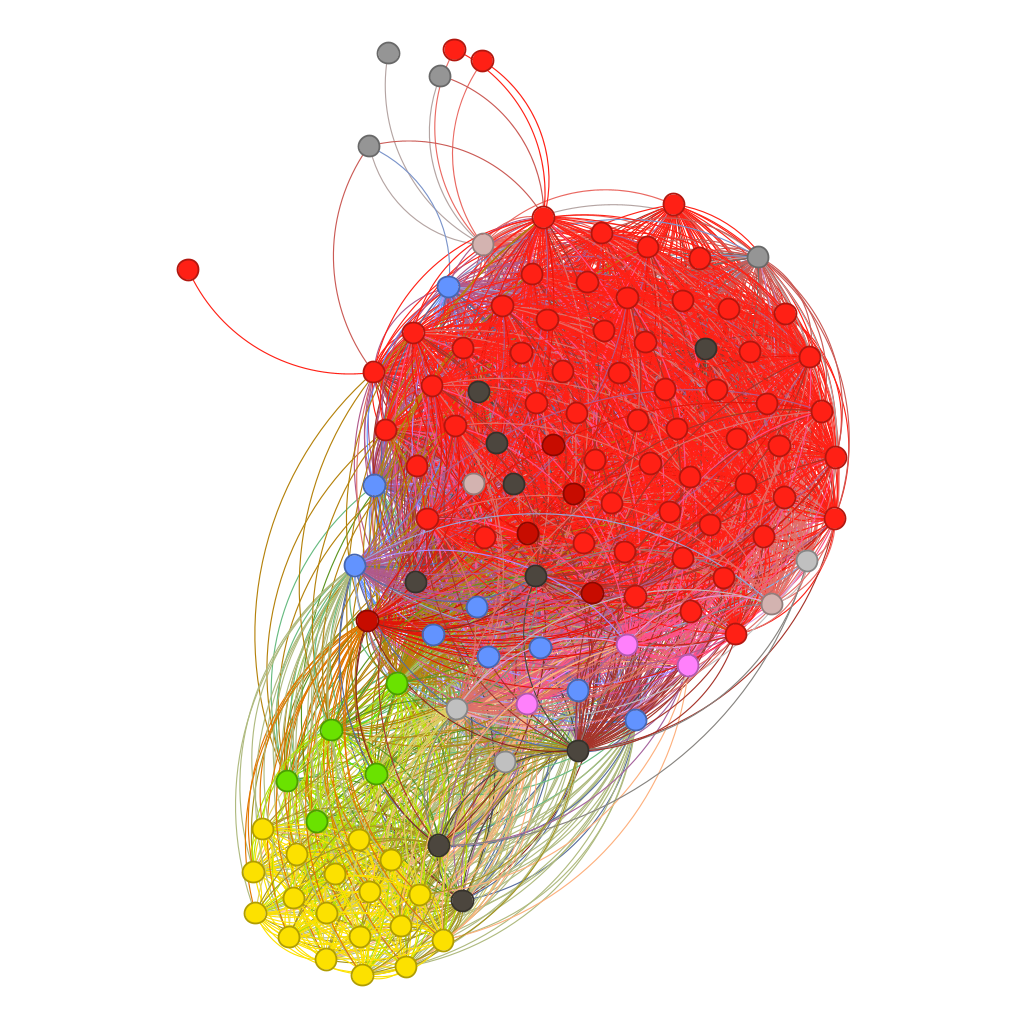
\includegraphics[width=\linewidth]{img/xvii_graph.png}
  \caption{Network of the XVII legislature. Different colors represent different political groups. Isolated nodes are not shown for visualization purposes.}
  \label{fig:graph}
\end{figure}


\begin{figure}[h]
  \centering
  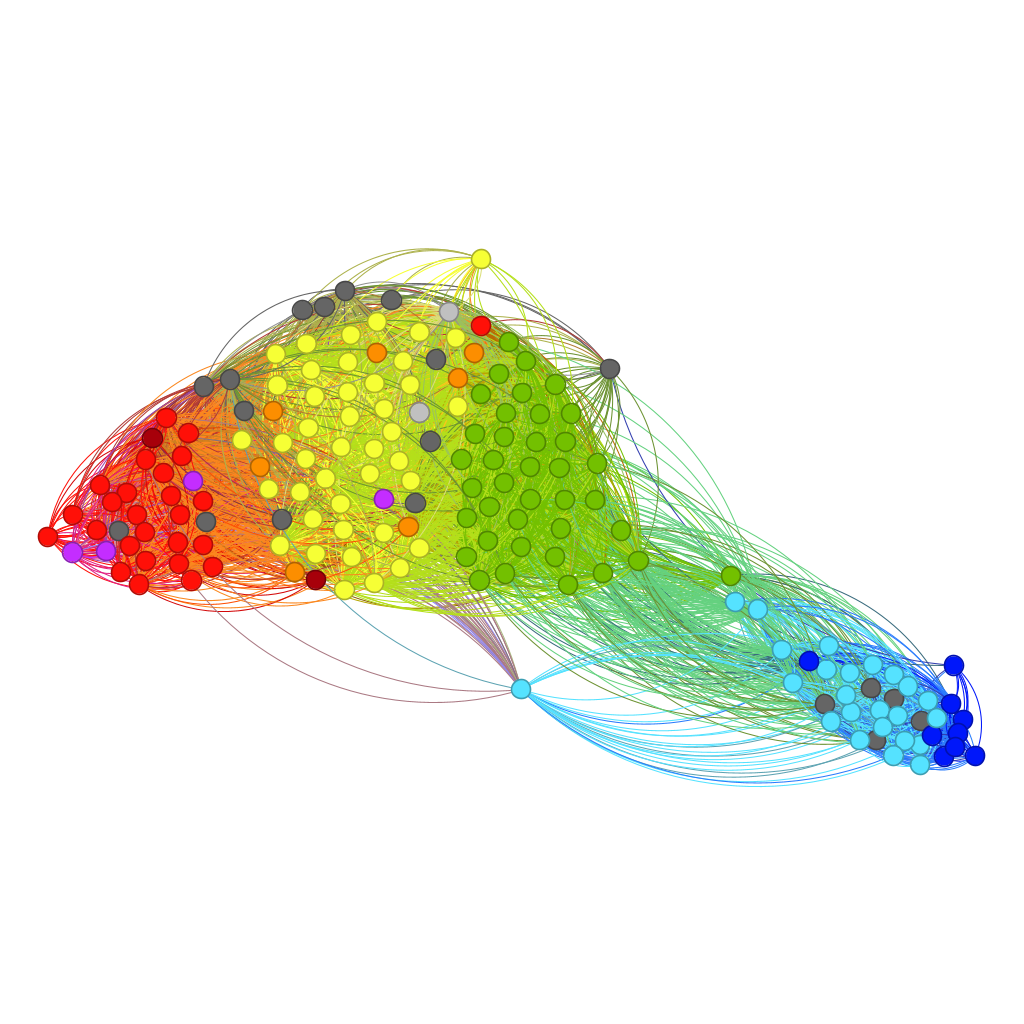
\includegraphics[width=\linewidth]{img/xviii_graph.png}
  \caption{Network of the XVIII legislature. Different colors represent different political groups. Isolated nodes are not shown for visualization purposes.}
  \label{fig:graph}
\end{figure}


In this section we will study the basic features of our network. For this purpose we will focus on aggregated data over a whole legislature. Nodes are represented by the deputies, and edges are built based on their voting similarity.\\
From now on, let's consider the XVII legislature.

\subsubsection{Nodes}
Applying the discussed preprocessing, we remain with 136 nodes in our network.

\subsubsection{Edge characterization}
Let's see more in detail how the edges were built.\\
The possible outcomes for each vote were:
\begin{enumerate}
    \item Absent
    \item In favour
    \item Against
    \item Abstention
\end{enumerate}
The nodes of our network are the members of the Chamber.\\
We introduce a weighted edge between each couple of Deputies.\\
\newpage

The weight is the similarity between their voting behaviors (excluding absence) defined as:
\begin{equation}
    \text{Similarity} = \dfrac{\text{\#same vote}}{\text{\#different vote + \#same vote}}
\end{equation}

Note that we only consider the votes in which both Deputies were present.
 We end up with a weighted graph.\\


\begin{figure}[h]
  \centering
  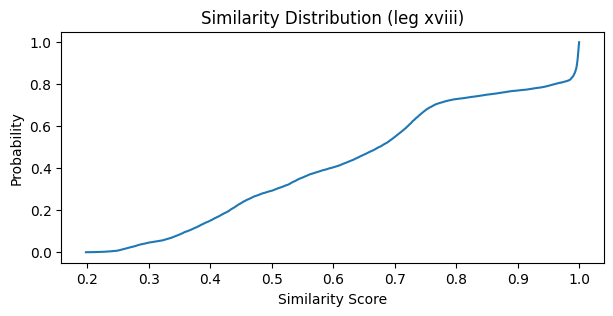
\includegraphics[width=\linewidth]{img/similarity_xvii.png}
  \caption{CDF for the similarity between nodes of the XVII legislature.}
  \label{fig:cdf}
\end{figure}

Now we want to introduce a threshold for the similarity and drop the edges which fall below it.
To define the threshold, let's consider the cumulative distribution function of the similarity (fig. \ref{fig:cdf}).
We decided to set our threshold in correspondence of the 50th percentile (median), considering only edges whose similarity value was above this value.\\
In the case of the XVII legislature,
 this corresponds to considering only edges with similarities above approximately 0.35.\\
Doing this, we pass from 9052
 to 4568 edges.


At this point, for simplicity, we drop the edge weights to work with an unweighted graph.\\

\subsection{Network Analysis}


Let's now analyze some basic features of our network: in table (\ref{tab:basic_measures}) we present an overview of the basic measures year by year.
It's important to note, that in the years $2015$ and $2016$ the networks are smaller, however, most of the metrics remain roughly stable throughout the years. The networks have all the same density more or less (by construction), and they have an extremely high average value of clustering coefficient. It's interesting to note that most of the networks have a single connected component.\\

As we said, from now on we focus on aggregated data of the XVII legislature.
\subsubsection{Degree distribution analysis} Let's now focus on the degree distribution of our network.
\begin{figure}[h]
  \centering
  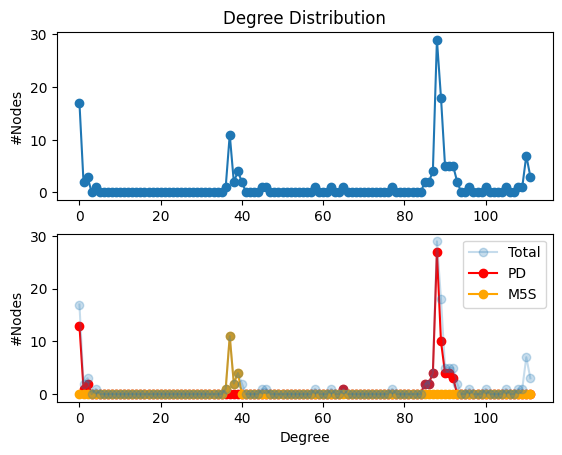
\includegraphics[width=\linewidth]{img/degree_xvii_party.png}
  \caption{Degree distribution of the network of the XVII legislature. In the bottom subplot, we consider the degree distributions separating members of the two main parties in the Chamber.}
  \label{fig:degree_distrib}
\end{figure}

Since we have a limited number of nodes, it is difficult to recognize a specific pattern.\\
If we look at figure (\ref{fig:degree_distrib}), apart from the peak at 0 (corresponding to 17 isolated nodes), we identify a peak around degree 40 and another around 90. These two peaks correspond to the two main political groups in the Chamber during the XVII legislature: M5S and PD. Their members, in general, voted similarly to the extent that also their degree is the same or nearly so.\\
The average degree is 67. Showing in general a high degree of connectivity.\\

In our analysis, as stated before, we set our edge threshold in correspondence with the median (in the case of the XVII legislature it corresponds to 0.35). However, it is interesting to study how the average degree changes if we change the edge threshold.
We can visualize that in figure (\ref{fig:degree_thresh}). Note that on the x axis we consider 50 linearly spaced thresholds from 0 to 1. 

\begin{figure}[h]
  \centering
  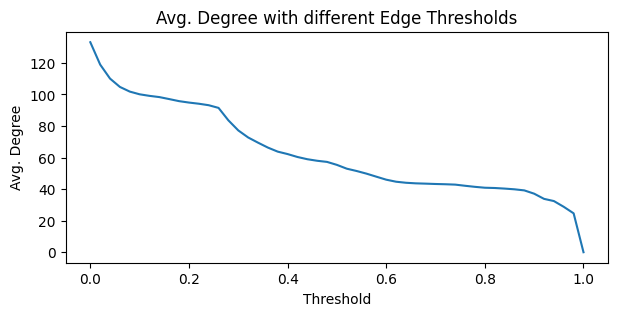
\includegraphics[width=\linewidth]{img/degree_xvii_varing_tresh.png}
  \caption{Average degree of the network of the XVII legislature, varying the applied edge threshold.}
  \label{fig:degree_thresh}
\end{figure}

As expected, increasing the threshold leads to a decreasing number of edges in the network. As an immediate consequence, the average degree decreases.

\subsubsection{Connected components analysis}

Excluding the isolated nodes (in this case 17), in the network we can identify a single connected component. It means that, with the selected threshold for similarity, bridges between different communities are maintained, and there is no complete segregation of parties.\\
Let's study how the situation changes varying the threshold, in figure (\ref{fig:conn_comps_thresh}).

\begin{figure}[h]
  \centering
  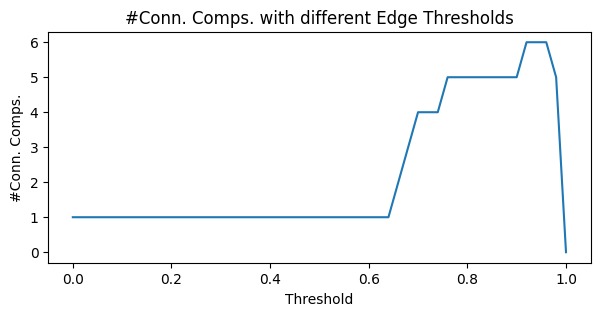
\includegraphics[width=\linewidth]{img/conn_comps_changing_thresh.png}
  \caption{Number of connected components of the network of the XVII legislature, varying the applied edge threshold.}
  \label{fig:conn_comps_thresh}
\end{figure}

We see that after a certain value (around 0.6) the number of connected components starts to increase. That is related to the decreasing number of edges in the network, that will eventually affect bridges between different connected components.

\subsubsection{Path analysis}
The average shortest path length is 1.37, while the network diameter is 3.
Both these measures display a densely connected graph.
The former measures the typical distance between pairs of nodes, and in this case it is rather small. The latter is a measure of the maximum number of edges needed to connect two nodes in the network. With a value of 3, it emphasize the dense nature of our network. 

\subsubsection{Clustering Coefficient, Density Analysis}

The average clustering coefficient is 0.80, while the density of the network is 0.50.\\
The average clustering coefficient provides insights into the connectivity of our network. It has a pretty high value, implying a general tendency to aggregation.\\
Note that the density is 0.50 by construction, since we decided to set the threshold for edges in correspondence of the median of the similarity.\\
In figure (\ref{fig:cc_dens_thresh}) we show how these properties change varying the threshold.\\

\begin{figure}[h]
  \centering
  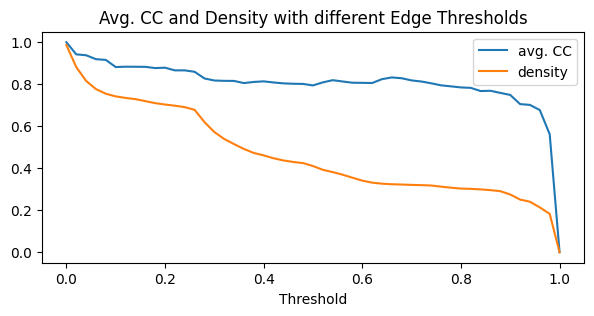
\includegraphics[width=\linewidth]{img/cc_density_xvii_varing_tresh.png}
  \caption{Average Clustering Coefficient and density of the network of the XVII legislature, varying the applied edge threshold.}
  \label{fig:cc_dens_thresh}
\end{figure}

We see that the average clustering coefficient is stable around 0.8-0.9 (except from when the threshold is 1 which means there are no edges in the graph). This means that the tendency to form local neighborhoods does not depend on the similarity threshold applied.\\
Of course, the density decreases while the threshold increases because we are removing more and more edges from the graph.

\subsubsection{Centrality analysis}
We now want to study some centrality properties of the network.\\
In particular we focus on Betweenness Centrality and Closeness Centrality of nodes, whose distributions are reported in figure (\ref{fig:centrality}).\\

Betweenness centrality is related to how much a node helps the network to remain connected. Since the network is pretty dense, values of betweenness centrality are all very close to 0.\\

Closeness centrality is related to the average distance between a node and all the other nodes in the network. Apart from isolated nodes (with CC = 0), we note that almost all nodes have a closeness centrality greater than 0.4, and most of them have values around 0.7. This shows that members of the Chamber are generally very close between them, in terms of voting behavior.
\begin{figure}[h]
  \centering
  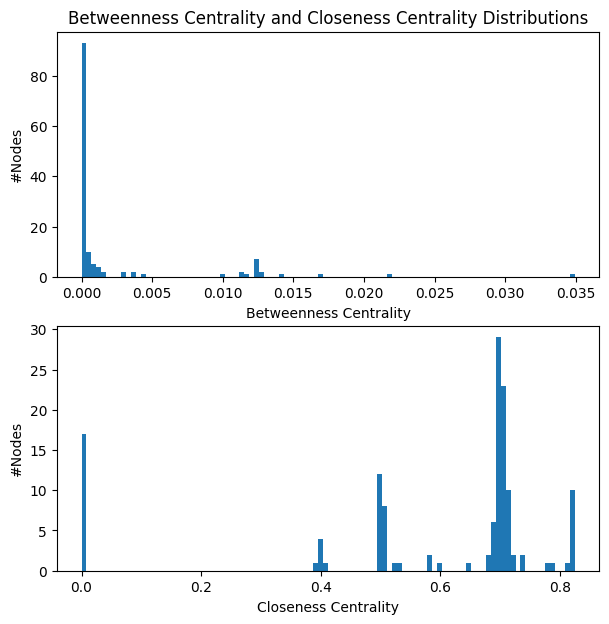
\includegraphics[width=\linewidth]{img/centrality_xvii.png}
  \caption{Betweenness Centrality (top) and Closeness Centrality (bottom) distributions for the network of the XVII legislature.}
  \label{fig:centrality}
\end{figure}

\subsection{Comparision with ER}
Let's now compare our graph with a random one.
To do that, we generate an ER graph with the same number of nodes as our graph, in our case 136. We also want our ER graph to have a similar number of edges to our real graph. To do so, we choose the value of p (probability of the presence of an edge between two nodes) according to the following relation:
\begin{equation}
    p = \dfrac{2 L}{N(N-1)}
\end{equation}
where N is the number of nodes and L is the number of edges.\\
In our case N = 136 and L = 4568, so we have p = 0.50. \\
In table (\ref{tab:er_ba}) we compare some of the basic measures computed on the ER graph, with the ones computed on our real network.
\begin{table}[h]
\begin{tabular}{lrrr}
\hline
               &    Real &      ER &      BA \\
\hline
 \#nodes        &  136 &  136 &  136 \\
 \#edges        & 4568  & 4570 & 4615 \\
 avg degree    &   67.18 &   67.21 &   67.87 \\
 \#isol. nodes  &   17 &    0 &    0 \\
 \#conn. comps. &    1 &    1 &    1 \\
 avg SPL       &    1.37 &    1.50 &    1.50 \\
 diameter      &    3 &    2 &    2 \\
 avg CC        &    0.80 &    0.50 &    0.72 \\
 Density       &    0.50 &    0.50 &    0.50 \\
\hline
\end{tabular}
\caption{Comparison of basic measures with ER and BA graphs.}
\label{tab:er_ba}
\end{table}

We note that the average degree of the ER graph is comparable to the one of our network. However, the degree distribution is pretty different, as we can see in figure (\ref{fig:degree_er}).

\begin{figure}[h]
  \centering
  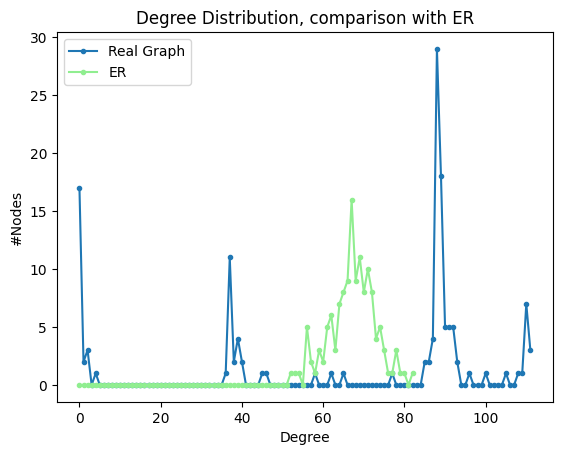
\includegraphics[width=\linewidth]{img/degree_dist_er_xvii.png}
  \caption{Degree Distribution: comparison between real graph and ER graph.}
  \label{fig:degree_er}
\end{figure}


The number of connected components, excluding isolated nodes, is the same. There is no significative difference in the average shortest path length either.\\
The diameter of the ER graph is 1 unit smaller than the real one; this is due to the fact that in the ER graph the connections are random, while in the real graph not all connections have the same probability to establish. For example, the path between two members of the Chamber with opposite political views will not be of length one, but will probably pass through one (or more) moderate member(s). This will make the network diameter wider with respect to the random scenario.\\

The average clustering coefficient of the random graph is significantly smaller than the one of the real graph. This highlights how the real network is, indeed, clustered.\\

Having almost the same number of edges, density is of course the same.


\subsection{Comparision with BA}

Finally, we compare our network with a Barabasi Albert graph. The BA graph is characterized by a scale-free topology with a power-law degree distribution. It is described by the (integer) parameter $m$, which determines the number of edges a new node forms with existing nodes during the growth process.\\
We chose for $m$ a value so that the number of edges of the BA graph was comparable with the number of edges of the real graph. In our case we have $m = 65$.\\

In table (\ref{tab:er_ba}) we compare some of the basic measures computed on the BA graph, with the ones computed on our real network, and on the ER graph.\\

We can see that the global properties of the BA network expressed in table (\ref{tab:er_ba}) are in line with the ones of the real graph. We note that the average SPL is slightly higher in the BA graph, and the average clustering coefficient is slightly smaller. This means that the level of clustering in our real network is, on average, greater than the scale-free case.\\
Finally, as we saw in the ER case, also in the BA graph the diameter is slightly smaller than the real case.\\

In figure (\ref{fig:degree_ba}) we plot the degree distribution of the BA graph compared with the real one. We see that the BA distribution does not capture the two peaks of the real one.\\

In conclusion, neither the ER model nor the BA model can capture the structure of the degree distribution of our network.

\begin{figure}[h]
  \centering
  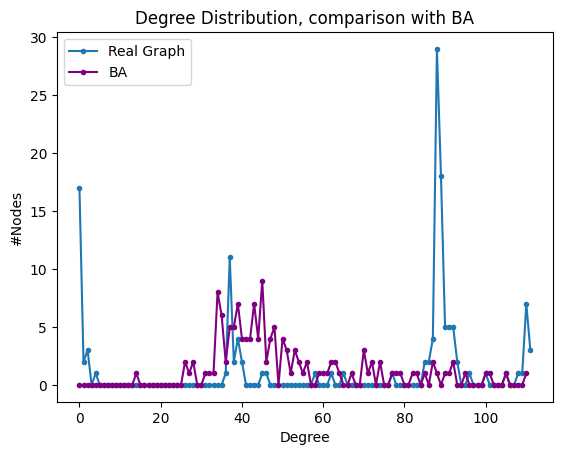
\includegraphics[width=\linewidth]{img/degree_dist_ba_xvii.png}
  \caption{Degree Distribution: comparison between real graph and BA graph.}
  \label{fig:degree_ba}
\end{figure}


%-----------------------


\section{Community Detection}
Party systems can be characterized based on their fragmentation and polarization. Party fragmentation corresponds to the number of parties existing in a political system, while polarization is related to the multiple opinions that lead to the division of members into groups with distinct political ideologies.\\
It's not uncommon that in fragmented systems the multiple political parties often make coalitions, or alliances, to reach a common end. Thus, a great amount of ideological similarity, expressed by the voting decisions, is observed across different parties, generating ideological communities \cite{AnIdeoComm}.\\

\begin{table*}[h]
\begin{tabular}{c|cccc|ccccc|ccccc|}
\cline{2-15}
                                 & \multicolumn{4}{c|}{\textbf{Louvain}} & \multicolumn{5}{c|}{\textbf{Angel}} & \multicolumn{5}{c|}{\textbf{K-Clique}} \\ \hline
\multicolumn{1}{|c|}{\textbf{Year}} &
  \textbf{\begin{tabular}[c]{@{}c@{}}\# of \\      Comm.\end{tabular}} &
  \textbf{Mod.} &
  \textbf{\begin{tabular}[c]{@{}c@{}}Avg.\\      PD\end{tabular}} &
  \textbf{\begin{tabular}[c]{@{}c@{}}SD\\      PD\end{tabular}} &
  \textbf{\begin{tabular}[c]{@{}c@{}}Merging \\ Thr.\end{tabular}} &
  \textbf{\begin{tabular}[c]{@{}c@{}}\# of \\      Comm.\end{tabular}} &
  \textbf{Mod.} &
  \textbf{\begin{tabular}[c]{@{}c@{}}Avg.\\      PD\end{tabular}} &
  \textbf{\begin{tabular}[c]{@{}c@{}}SD\\      PD\end{tabular}} &
  \textbf{K} &
  \textbf{\begin{tabular}[c]{@{}c@{}}\# of \\      Comm.\end{tabular}} &
  \textbf{Mod.} &
  \textbf{\begin{tabular}[c]{@{}c@{}}Avg.\\      PD\end{tabular}} &
  \textbf{\begin{tabular}[c]{@{}c@{}}SD\\      PD\end{tabular}} \\ \hline
\multicolumn{1}{|c|}{2013}       & 4     & 0.21     & 0.74     & 0.14    & 0      & 4  & 0.21  & 0.74  & 0.14  & 2     & 4   & 0.21   & 0.74   & 0.14   \\
\multicolumn{1}{|c|}{2014}       & 4     & 0.21     & 0.73     & 0.11    & 0      & 3  & 0.20  & 0.75  & 0.13  & 3     & 4   & 0.20   & 0.73   & 0.13   \\
\multicolumn{1}{|c|}{2015}       & 3     & 0.20     & 0.70     & 0.11    & 0.21   & 3  & 0.20  & 0.70  & 0.11  & 4     & 3   & 0.20   & 0.70   & 0.11   \\
\multicolumn{1}{|c|}{2016}       & 4     & 0.15     & 0.68     & 0.13    & 0      & 3  & 0.14  & 0.65  & 0.12  & 2     & 4   & 0.15   & 0.68   & 0.13   \\
\multicolumn{1}{|c|}{2017}       & 3     & 0.23     & 0.69     & 0.11    & 0.64   & 3  & 0.20  & 0.69  & 0.10  & 13    & 3   & 0.23   & 0.69   & 0.11   \\
\multicolumn{1}{|c|}{2018-xvii}  & 3     & 0.24     & 0.69     &         & *      & *  & *     & *     & *     & 11    & 4   & 0.01   & 0.67   & 0.27   \\
\multicolumn{1}{|c|}{2018-xviii} & 2     & 0.41     & 0.70     & 0.13    & 0.07   & 2  & 0.41  & 0.70  & 0.13  & 3     & 2   & 0.41   & 0.72   & 0.13   \\
\multicolumn{1}{|c|}{2019}       & 3     & 0.25     & 0.70     & 0.14    & 0.93   & 2  & 0.11  & 0.70  & 0.14  & 2     & 1   & 0      & 0.70   & 0.14   \\
\multicolumn{1}{|c|}{2020}       & 2     & 0.46     & 0.72     & 0.14    & 0.07   & 2  & 0.46  & 0.71  & 0.14  & 3     & 2   & 0.46   & 0.71   & 0.14   \\
\multicolumn{1}{|c|}{2021}       & 2     & 0.27     & 0.68     & 0.13    & 1      & 1  & 0.11  & 0.67  & 0.11  & 2     & 2   & 0.02   & 0.68   & 0.13   \\
\multicolumn{1}{|c|}{2022}       & 2     & 0.22     & 0.75     & 0.10    & 1   & 2  & 0.03  & 0.71 & 0.10  & *     & *   & *      & *      & *      \\ \hline
\end{tabular}
\caption{Community detection results obtained for different algorithms. Note: we couldn't calculate the values marked by * due to problems in the convergence of algorithms.}
\label{tab:community}
\end{table*}


Table \ref{tab:community} shows the results of different community detection algorithms on the yearly networks. The algorithms adopted for the search of communities were Louvain, Angel, and K-clique.\\

We decided to use different algorithms to exploit the differences between the communities found, since each algorithm has its definition of community.\\

After a very quick tuning phase, we decided to set the merging threshold of Angel independently for each year. We defined some candidates values, $\{0, 0.07, 0.14, 0.21, 0.28, 0.35,\\ 0.42, 0.5, 0.57, 0.64, 0.71, 0.78, 0.85, 0.92, 1\}$, and selected the value associated to the highest modularity. We also ignored the communities with less than $4$ nodes. \\

Similarly, for the k-clique algorithm we decided to range the size from $2$ to $15$ and select, for each network, the value associated with the highest modularity score.\\

We decide to use the modularity score to evaluate the communities structure, and an external measure that fits our case study, the \textit{Partisan Discipline} metric \cite{PD}.
 This metric captures the ideological alignment of a member to his party (or his community). Given a member \textit{x}, the \textit{Partisan Discipline} of \textit{x} is given by the fraction of all voting sessions where \textit{x} voted in the same way as the majority of the member in his party (or his community). 
\begin{equation}
    p = \dfrac{\sum_{i = 1}^{n}{I(x, p_{x,i})}} {n}
\end{equation}

\noindent Where $I(x, p_{x,i})$ is 1 if \textit{x} voted in the same ways as its party (or community) in the same voting session, $0$ otherwise, and \textit{n} is the total number of voting sessions.
 It can range from 0 to 1, where 1 indicates that a member is cohesive and 0 otherwise.\\

A common result between the algorithms is the fact that the number of communities found is always much smaller than the total number of parties, which is $12$ before $2017$, $10$ after, confirming the fragmentation and ideological overlap of multiple parties.\\

\begin{table}[h]
\begin{tabular}{ccclll}
\multicolumn{1}{c|}{Party}    & Community 1          & Community 2          &  &  &  \\ \cline{1-3}
\multicolumn{1}{c|}{SI}       & 0.05                 & 0                    &  &  &  \\
\multicolumn{1}{c|}{CI}       & 0.02                 & 0                    &  &  &  \\
\multicolumn{1}{c|}{PD}       & 0.23                 & 0                    &  &  &  \\
\multicolumn{1}{c|}{IPF-IC}   & 0.06                 & 0                    &  &  &  \\
\multicolumn{1}{c|}{M5S}      & 0.40                 & 0.01                 &  &  &  \\
\multicolumn{1}{c|}{IV-IC'E'} & 0.07                 & 0                    &  &  &  \\
\multicolumn{1}{c|}{LEGA}     & 0                    & 0.50                 &  &  &  \\
\multicolumn{1}{c|}{FI}       & 0.01                 & 0.25                 &  &  &  \\
\multicolumn{1}{c|}{FDI}      & 0                    & 0.18                 &  &  &  \\
\multicolumn{1}{c|}{MISTO}    & 0.16                 & 0.06                 &  &  &  \\
\multicolumn{1}{l}{}          & \multicolumn{1}{l}{} & \multicolumn{1}{l}{} &  &  & 
\end{tabular}
\caption{Proportion of political parties member inside the different communities extracted using Louvain algorithm for the 2020 voting sessions.}
\label{tab:community_party}
\end{table}

The average \textit{Partisan Discipline} of these communities is very close, or slightly worse, to the average computed using the original parties. Also, the standard deviation of the \textit{Partisan Discipline} is almost every time lower in the communities than in original parties. Overall, members are disciplined with respect to the voting preferences of the parties, and the resulting communities are quite cohesive in their voting patterns. \\

In contrast, the topological structure of the identified communities, expressed with the \textit{modularity} score, is in general weak.\\ Independently from the algorithm used, in $2020$ the communities have the highest modularity, a moderate value that tells us that there is a discernible separation between communities in terms of their internal connectivity. We may hypothesize that this can be related to the Covid-19 emergency, which created a stronger distinction between communities.\\
Then, starting from the following year, the modularity decreases, stabilizing itself with similar values of the previous years using Louvain, while using Angel and K-clique the values fall and reach almost zero, indicating similarities across members of different communities.\\
This happens despite the moderately large average party discipline maintained by the communities. 

That is, the two selected metrics (Modularity and average PD) provide different views of the political scenario.\\



In general, the communities found with Angel and K-clique vary in \textit{modularity} more than the ones found with Louvain, and with both algorithms we found at least a network with a single community. With Louvain, instead, we have a more stable situation, where the number of communities doesn't affect the \textit{modularity}, which is stable around $0.2$ in most of the cases.\\

It is interesting to study how the identified communities are composed in terms of political parties. In table \ref{tab:community_party} we consider, as an example, the year 2020, where the Louvain algorithm identifies 2 distinct communities. We analyze what political parties compose these coalitions, and in what proportion.\\
The distinction between the center-left and the center-right block is evident, with a virtually negligible overlap.\\ 

To sum up, in our study we found that several parties can be grouped in few communities, characterized by disciplined members. The topological strength of communities, represented by the modularity score, is moderate, and depends on the year considered. The cohesiveness of identified communities, expressed by the average party discipline, is high and tends to remain more stable.


\section{Stream Graph}

The network we are studying is very dynamic. Opinions may change over time, and different coalitions may emerge between members of the Chamber. The changes in voting behavior may have different origins, and thus they can emerge in different timescales.\\
For this reason, it is useful to study our network from a \textit{Stream Graph} point of view.\\
Using the \textit{DyNetX} library, we create a stream graph using months as temporal snapshots.\\
For every month we create our snapshot network following the approach described at the beginning of the article. However, to have less variability in the number of nodes, we decided not to eliminate the \textit{"serial absent"} members.\\
There is still a slight variability in the number of nodes, due to the fact that data from certain members were missing in certain months.\\ Moreover, no data was available for some months (Jan-May 2018, Jan 22, Sept 22, and Oct 22); those months are not reported in the analysis.\\

For the XVII legislature, we end up with a stream graph with 600 nodes and 179421 interactions.
For the XVIII, we have a total of 615 nodes and 188783 interactions.\\

To analyze the stability of the temporal graph, we focus on monthly temporal snapshots, studying the following features evolving over time:
\begin{itemize}
    \item Number of Nodes and  Interactions (Figure \ref{fig:dynamic_nodes_edges})
    \item Average Clustering Coefficient and Average Degree (Figure \ref{fig:cc_deg})    
    \item Number of communities identified using Louvain and corresponding modularity (Figure \ref{fig:dynamic_louvain})
    \item  Average Party Discipline (Figure \ref{fig:dynamic_apd})
\end{itemize}

\begin{figure*}[h]
  \centering
  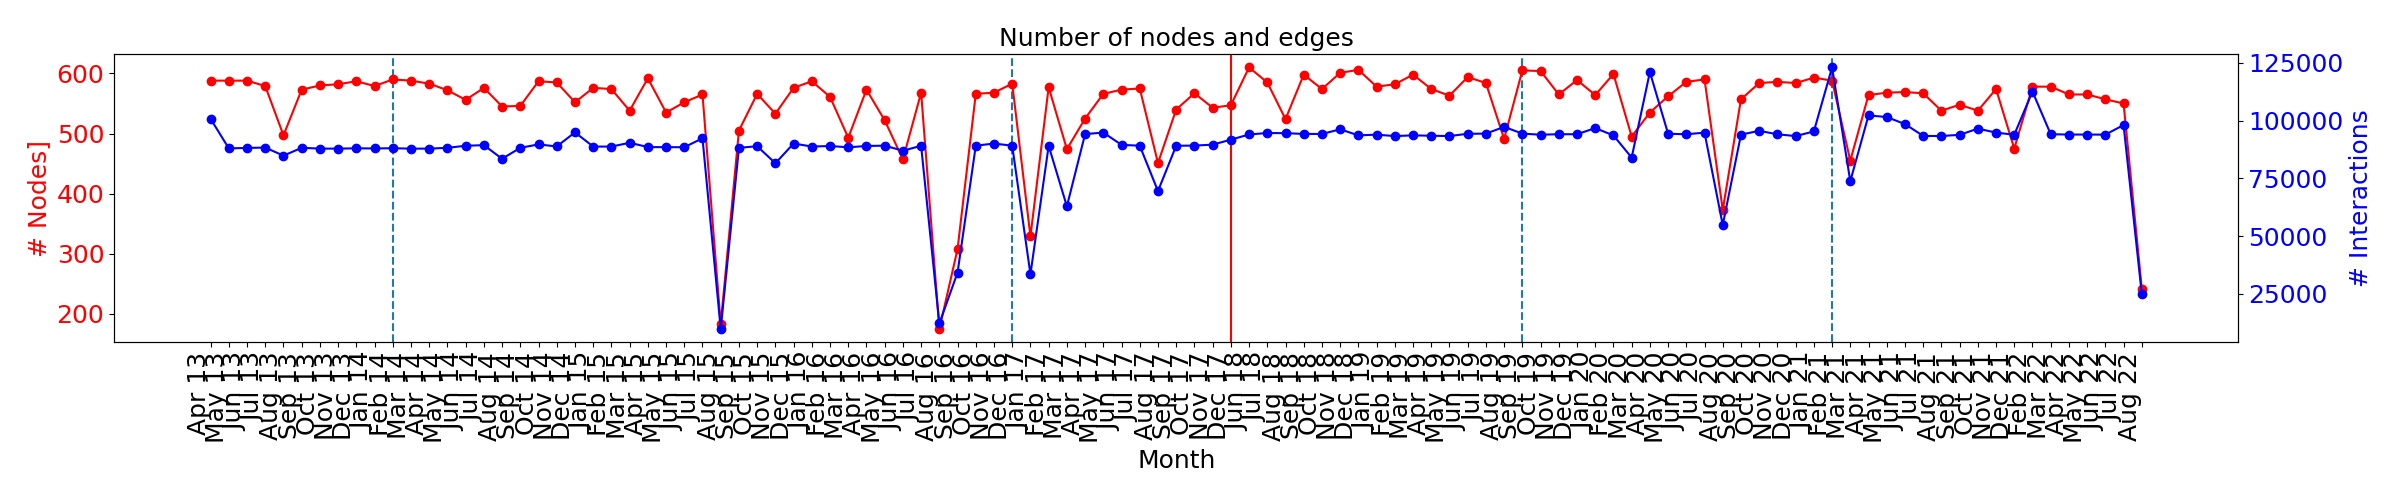
\includegraphics[width=\linewidth]{img/dynamic_nodes_edges_tot.png}
  \caption{Number of Nodes (red) and Interactions (blue) across different months of XVII and XVIII legislatures.}
  \label{fig:dynamic_nodes_edges}
\end{figure*}



\begin{figure*}[h]
  \centering
  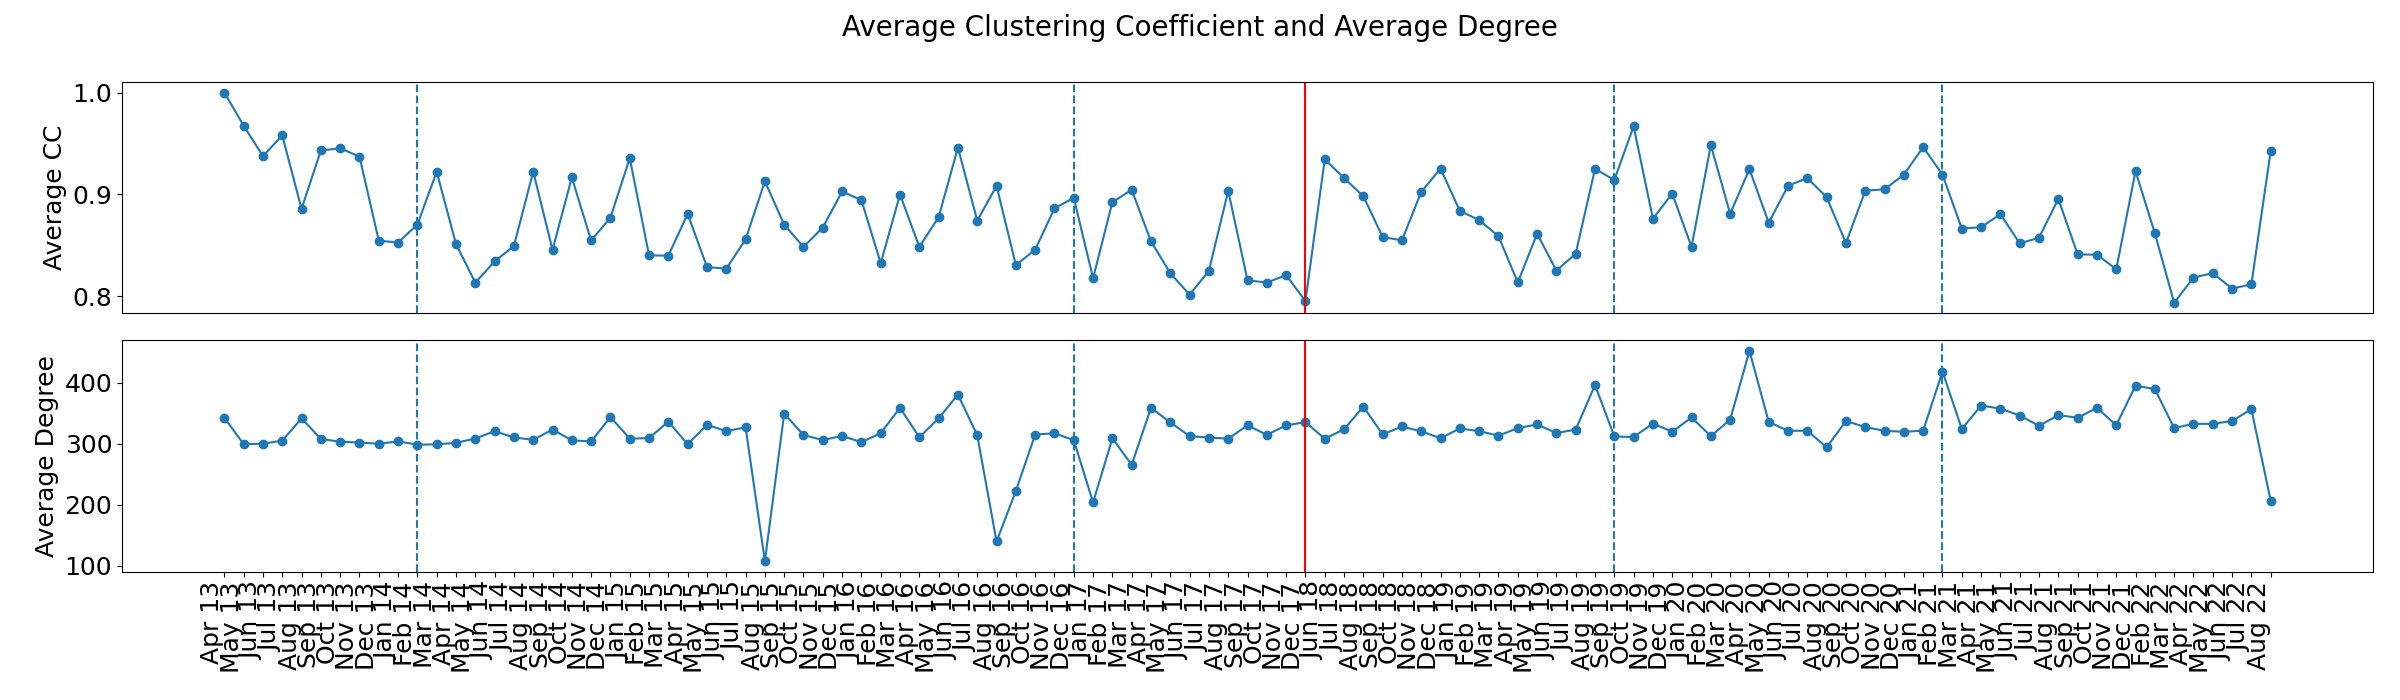
\includegraphics[width=\linewidth]{img/dynamic_avg_cc_deg_tot.png}
  \caption{Average CC (top) and Average degree (bottom).}
  \label{fig:cc_deg}
\end{figure*}

\begin{figure*}[h]
  \centering
  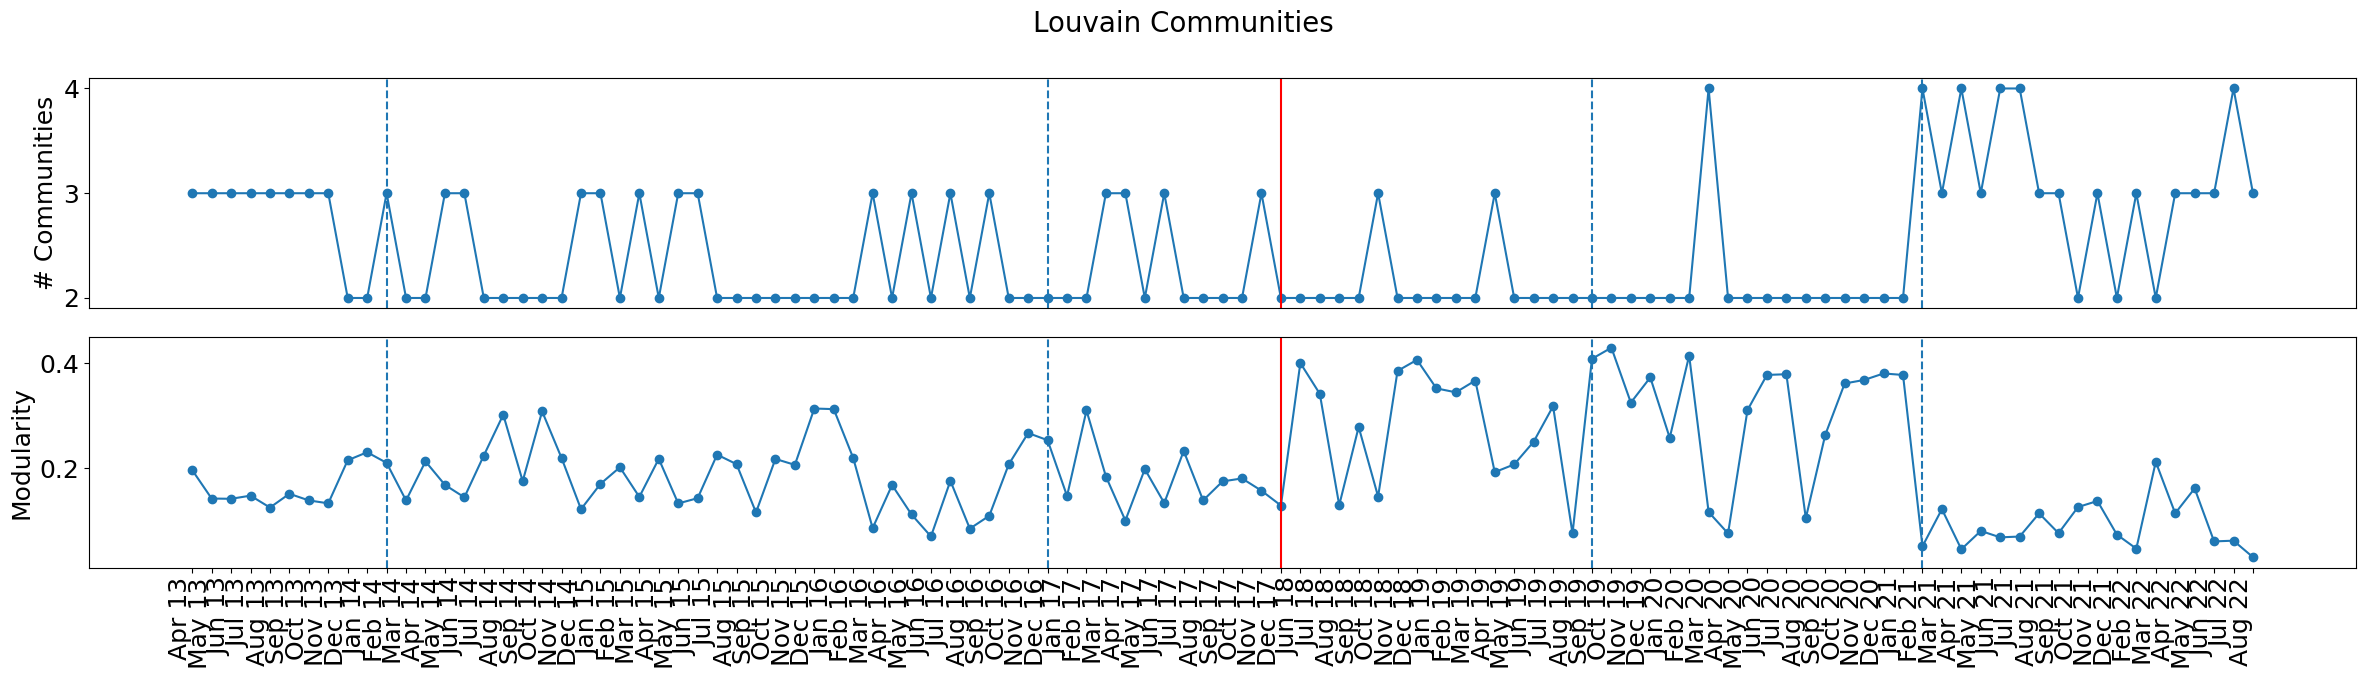
\includegraphics[width=\linewidth]{img/dynamic_louvain_tot.png}
  \caption{Number of Louvain Communities (top) and corresponding modularity (bottom).}
  \label{fig:dynamic_louvain}
\end{figure*}



\begin{figure*}[h]
  \centering
  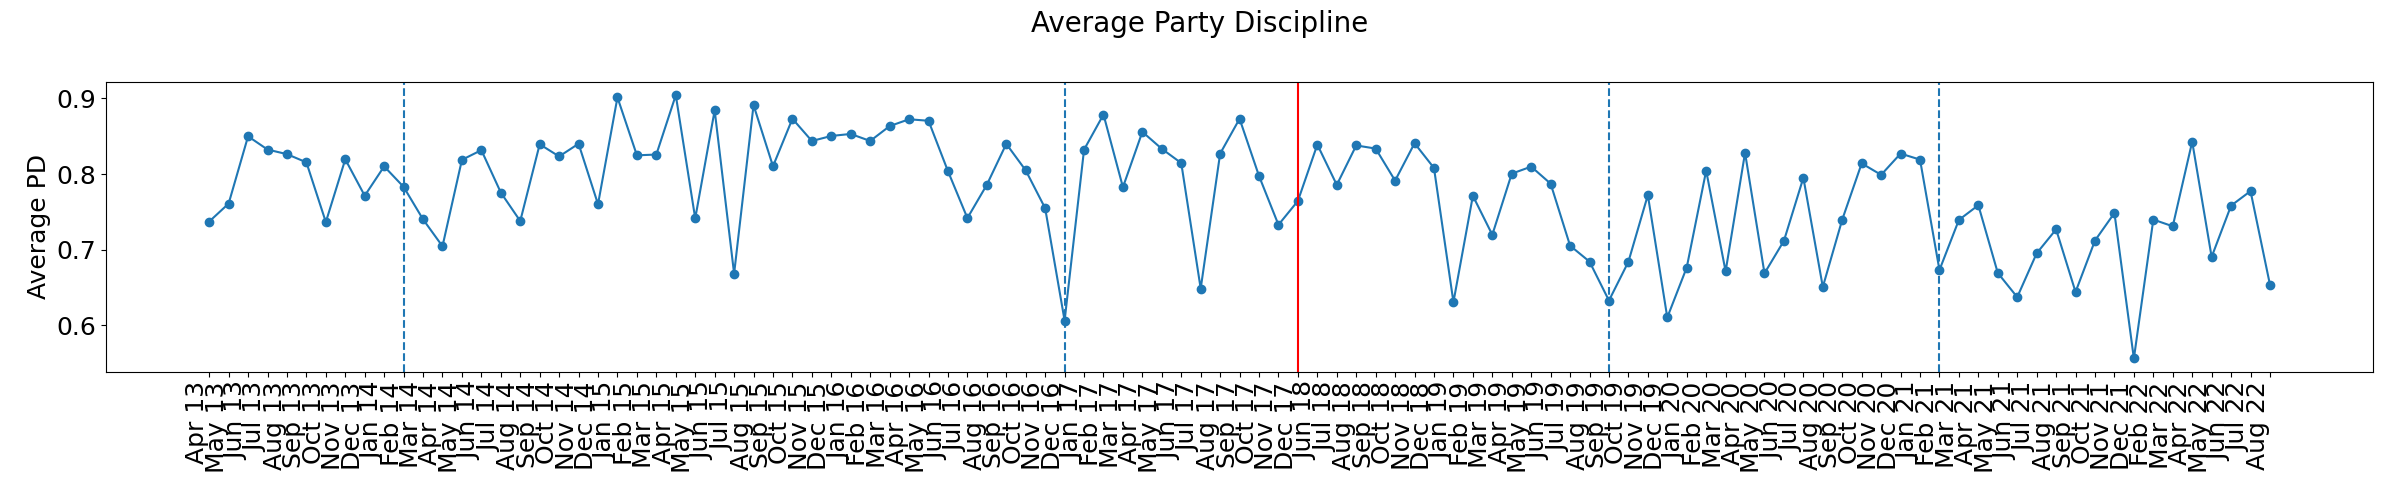
\includegraphics[width=\linewidth]{img/dynamic_apd_tot.png}
  \caption{Average Party Discipline score.}
  \label{fig:dynamic_apd}
\end{figure*}

In the figures, the vertical dashed lines correspond to months in which a new Prime Minister was appointed (and a new government formed); the red vertical line corresponds to the distinction between XVII and XVIII legislature.\\

In figure \ref{fig:dynamic_nodes_edges}, we see that the number of nodes of the network is quite stable, except for some months (typically August), where there is an evident lack of data.\\
The average number of nodes is 546, with standard deviation 77.\\
The number of edges follows a similar trend, with average 88281 and standard deviation 16621.\\
Since the average degree is the ratio between the number of edges and the number of nodes, it has a similar trend (320 $\pm$ 42).\\

The average clustering coefficient is pretty stable, showing small fluctuations across different months. In general, it has a high value (0.88 $\pm$ 0.04), indicating a high degree of clustering between members of the Chamber.\\

It is interesting to study the number of communities that are identified in different months (using Louvain). During the XVII legislature, we see that this number oscillates between 2 and 3. In the XVIII legislature, during the first two governments we almost always have a bipolar system, while during the last government the number of communities identified is more variable, ranging from 2 to 4.\\
As we have already seen with yearly data, the number of communities identified is smaller than the number of actual parties present in the Chamber. This highlights the ideological overlap of some parties.\\

The modularity score is a great indicator of how strong the communities found are from a topological point of view.
 Modularity computed over the Louvain communities shows a great variability: across all the months considered, it has a mean of 0.2 and a standard deviation of 0.1.\\
During the XVII legislature it fluctuates around 0.2, describing moderately structured communities.
 During the first two governments of the XVIII legislature, modularity scores reach higher values (up to around 0.4): in this period of time, communities are more strongly structured. Finally, during the last government of the XVIII legislature (from February 2021), modularity scores drop significantly: there is less distinction between different communities. This can be due to the "technocratic" nature of the government led by Mario Draghi, composed of members from various political parties, including both the center-left and center-right, as well as several independent technocrats. \\

Finally, the average party discipline captures how cohesive are different parties (on average). We see that this value is pretty high, showing in general an high cohesiveness. However, there are still some fluctuations between different months.\\

Overall, what we see is a network dominated by fluctuations in the main metrics. This is both due to the fast dynamics of political opinions and also to the incomplete availability of data. For this reason, it is hard to identify precise patterns in the network evolution.\\ 

%\clearpage





\section{Open question}
Now we would like to address the following question: "It is possible to classify months characterized by government crisis, only by using graph features?".\\
First, it's important to define what we are searching for. Italian politics is characterized by strong instability, the expected life for a government is 414 days, which becomes 380 days not considering the \textit{'sede vacante'} days, the period between the fall of a government and the start of a new one. Keeping this in mind, we tried to exploit the differences between the different months, using extracted data, to learn whether the voting patterns and the networks built from them can be used as predictors for an imminent crisis, and a consequent fall in the government.\\

The first problem encountered in this analysis was to precisely define how to label our month as a crisis (class 1) or not a crisis (class 0). 
The information regarding the month when a government officially ended is easily retrieved. However, we thought that the period of political instability could not be restricted to only that month.

That's why we decided to label it as '1' both the month before the fall of the government and the month after. We recognize that this was an arbitrary definition, and this would deserve a more in-depth study.\\
In the end we had $15\%$ of the entire dataset labeled as 1, the rest labeled as 0.\\

\begin{figure*}[h]
  \centering
  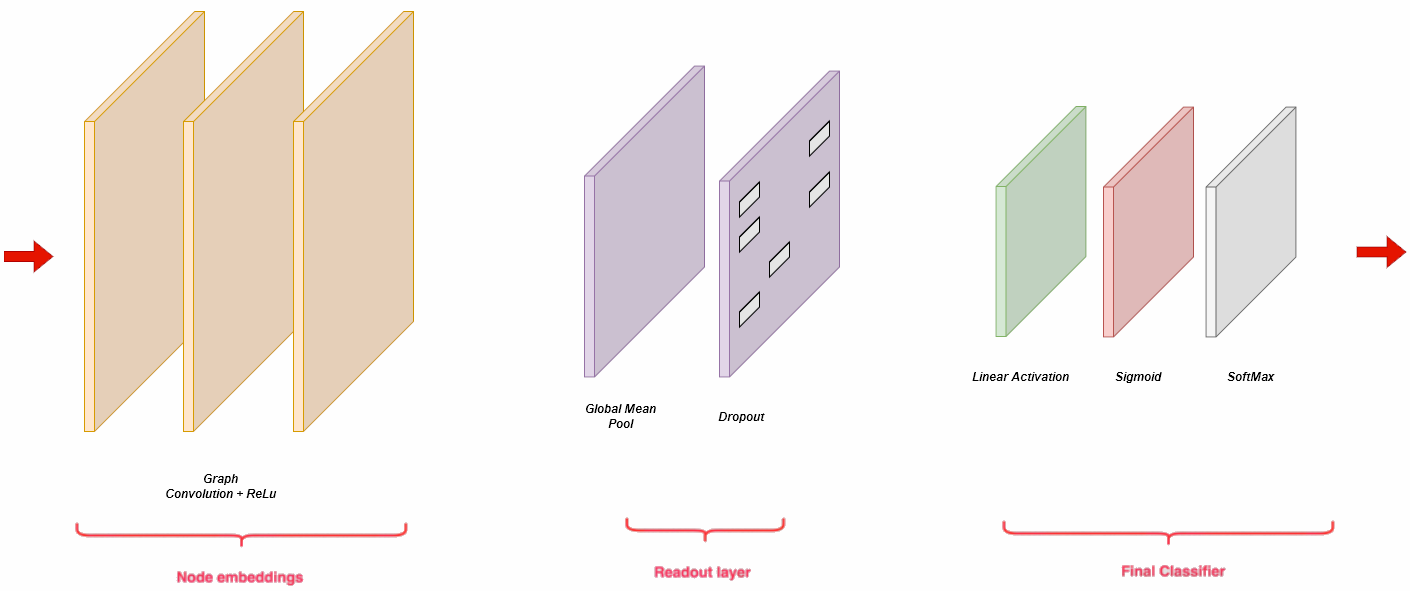
\includegraphics[width=0.9\linewidth]{img/nn scheme.png}
  \caption{Scheme of the GNN used for our graph classification task. First, we do a convolution, based on the adjacency matrix, in order to embed every node of the graphs. Then we use a global mean pool layer to aggregate node embeddings into a single graph embedding. Finally, we train a classifier to complete the task.}
  \label{fig:nn}
\end{figure*}

\subsection{Graph Neural Network}

Our main task was a binary classification one, we decided to build a Graph Neural Network (GNN) and classify each graph based on the information embedded in the structure.\\
The idea is to embed graphs based on their structural properties, in such a way so that they are linearly separable.\\

The first thing we did was prepare the dataset for the classification task.\\
To create a Graph dataset we followed the official documentation\footnote{\url{https://pytorch-geometric.readthedocs.io/en/latest/tutorial/create_dataset.html}} of \textit{Pythorch Geometric}.

After defining the labels for the graphs, we split the data into train and test, using a classical train-test split with stratification on the target variable. For the model evaluation, we trained our network using the binary categorical cross-entropy as loss function.\\
As input features, we used the adjacency matrix of the graph, automatically extracted by the \textit{PyG} library, and, for each node, we extracted some metrics to help the classification model in the task. In particular we used:
\begin{itemize}
    \item Node degree 
    \item Betweenness Centrality
    \item Closeness Centrality
    \item PageRank
    \item Eigenvector Centrality
\end{itemize}

Then we defined the structure of the GNN. Our model learns to classify graphs using three main steps (schematized in figure \ref{fig:nn}):
\begin{enumerate}
    \item Embed nodes using several rounds of message passing. In this case, we use three convolutions layers, each of which is followed by a ReLu layer.
    \item Aggregate these node embeddings into a single graph embedding (called readout layer). The average of node embedding is used (global mean pool).
    \item Train a classifier based on graph embedding. We decided to add a Dropout layer, setting p = 0.5, then a Sigmoid layer, and a final Softmax layer to extract the probability associated with each class.
\end{enumerate}
We divided the train set in batches, and start the training of our models, adding a regularization term to avoid overfitting. To avoid overtraining our model, we split the train set into train and validation, and, during training, the model is evaluated on a holdout validation set after each epoch. If the performance of the model on the validation set starts to degrade, then the training process is stopped. We defined a 'patience' parameter with a value of $15$. \\

After the first training session, the performance wasn't exciting, the loss in training was halved, but the accuracy in the testing phase was $0.25$. However, this value has not much meaning, since our classifier always predicts the same label.\\

We note that our dataset has a class imbalance: this may represent a problem because the model is unable to learn meaningful features from the data and predicts the majority class all the time.
 The optimizer finds a local minimum for the loss, corresponding to always predicting the class which is dominant in the dataset.\\

We decided to modify the loss function, accounting for the imbalanced scenario and weighting the classes based on the sample size for each class. Despite all our efforts, the performance didn't change. Our model did not recognize different patterns between crisis months and 'normal' months.\\


Another approach to solving the problem can be data augmentation: a first idea could be oversampling the minority class or undersampling the majority class.
 Another possibility is to synthetically create data of unbalanced classes which are similar to the existing ones.\\
We tried to undersample the majority class, creating a dataset with an equal number of 'crisis' and 'normal' months. However, also, in this case, the network could not learn from the data, predicting always 'crisis' or always 'normal'.\\

At this point we believe that a more fundamental problem could be happening: the graph structure and the node features we are considering are not informative enough. It can be the case that there are some other features that better capture the instability of the political scenario. Or simply it can be that there is not a significant correlation between the voting behaviors of Deputies and the government crisis.\\

One aspect of our classification approach is that it does not consider the previous history of the network, but tries to predict if a month is "of crisis" or not, just by considering the features of that specific month. Approaches that also consider the history of the network should be investigated, for example, a Recurrent Graph Neural network could be optimal for this scope.\\

Other strategies can be pursued as well, one involves the study of how can we define a government crisis, and how to convert the information in network structure, using the partisan discipline to add insights into the voting behavior. Moreover, one can focus on why the model fails to recognize different labels and, using explainability frameworks, discover what feature can contribute to the final classification.



%\section{Discussion}

Our dataset is composed of 107 graphs, one for each month. We want to embed those graphs based on their structural properties, in such a way so that they are linearly separable.\\
Each graph is given a label: '1' if it corresponds to a month of crisis, and '0' otherwise.\\

The data is divided into two datasets: a training set, which contains the first 89 months, and a test set, containing the remaining 28.\\


\clearpage
% The next two lines define the bibliography style to be used, and the bibliography file.
\bibliographystyle{ACM-Reference-Format}
\bibliography{biblio}

\end{document}
